\documentclass[a4paper,11pt]{article}
\setlength{\topmargin}{-.5in}
\setlength{\textheight}{9in}
\setlength{\oddsidemargin}{.125in}
\setlength{\textwidth}{6.25in}
\usepackage[pdftex]{graphicx}
\usepackage{fancyvrb}

\makeatletter
\renewcommand\paragraph{%
   \@startsection{paragraph}{4}{0mm}%
      {-\baselineskip}%
      {.5\baselineskip}%
      {\normalfont\normalsize\bfseries}}
\makeatother

\begin{document}

% The Title page
\begin{titlepage}
\begin{center}

\includegraphics[width=0.6\textwidth]{fig/logo}\\[3cm]    
\textsc{\LARGE Mapping the Via Appia in 4D}\\[0.5cm]
\textsc{\large Via Appia 4D GIS: Software User Manual}\\[0.5cm]
\vfill
\end{center}
{\large
\emph{O. Martinez-Rubi } \\
}
{\large
{Netherlands eScience Center, \\
Science Park 140 (Matrix 1), 1098 XG Amsterdam, the Netherlands\\
}
}
\begin{center}
{\large \today}
\end{center}
\end{titlepage}

\tableofcontents

\newpage


\section{Introduction}

In this project, an area full of funerary monuments or sites in the fifth and sixth miles of the Via Appia Antica is thoroughly studied. This is possible thanks to the new 4D GIS system which combines several types of data: point clouds in different resolutions, meshes, pictures, paintings and attributes information of the several monuments.

All the previous data can be visualized in the new eScience 4D GIS system that combines a 4D viewer with analysis tools of the University of Groningen and a database which contains the attribute data of multiple sites. The interaction between the viewer and the database allows the users to refine what data is visualized based on attributes selection. This system, which can be updated when new data is available, allows multiple researchers in different locations to analyse and study the area in 4D and aims to function as an example for other complex archaeological study areas.

% Outline
This document is the user manual for the new Via Appia 4D GIS system. Section \ref{sec:overview} gives an overview of the system. The Via Appia Linux server is described in Section \ref{sec:server}. The different types of data are detailed in Section \ref{sec:data} while in Section \ref{sec:db} you can find information regarding the used database. The main API is a 4D viewer with access to the database and it is detailed in Section \ref{sec:viewer}. %Finally, Section \ref{sec:python} contains the description of the Python scripts that perform the tasks related to the system. 

\section{Via Appia 4D GIS overview}
\label{sec:overview}
The developed 4D GIS system has a two-tier architecture. The server contains the master copy of the data and a PostgreSQL database called \textit{viaappiadb}. The clients download the data required for visualization and run the 4D viewer which connects to the remote database when required.

\begin{figure}[!ht]
\centering
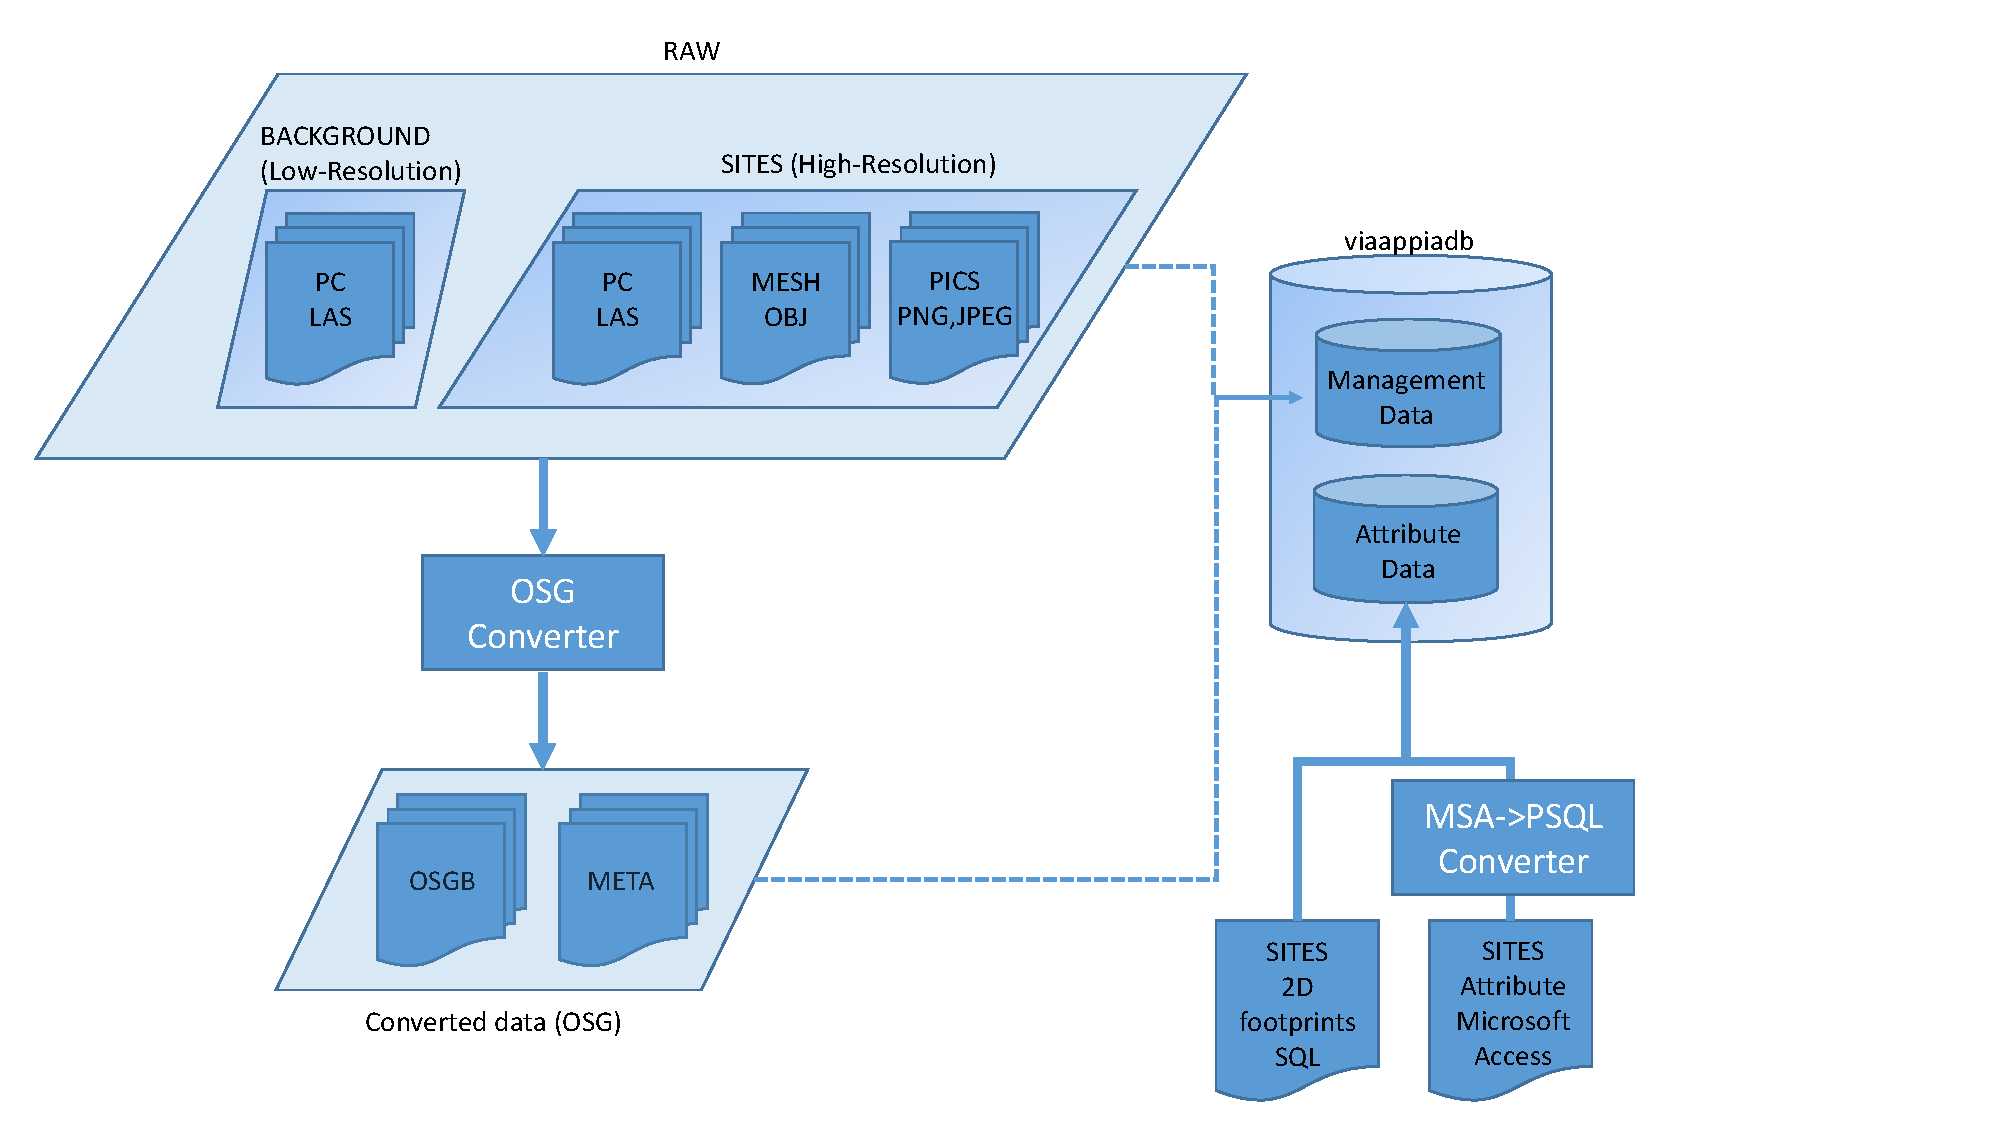
\includegraphics[scale=0.5]{fig/server_diagram.pdf}
\caption{Data preparation framework executed in the Via Appia Linux server.}
\label{fig-serverdiagram}
\end{figure}

A diagram of the data preparation framework which is executed in the server is shown in Figure \ref{fig-serverdiagram}. The raw data is converted to the OpenSceneGraph (http://www.openscenegraph.org) binary format. The \textit{viaappiadb} database is filled with meta-data information of the location of the raw data and the converted data. The archaeological information with attribute data for the several sites is provided in a Microsoft Access file. It needs to be converted to the PostgreSQL format before being imported into the main database. The footprints are provided in a PostgreSQL dump file and are imported into the \textit{viaappiadb} database as well.

Once the data preparation framework has been executed in the server the several clients can start using the 4D GIS system. The clients (Windows desktops or laptops) need to download local copies of the data required for visualization. The \textit{launcher} tool based on the Xenon library developed by the Netherlands eScience Center (NLeSC) is used for this purpose. The tool also downloads the configuration file required by the 4D viewer. Once both the data and the configuration file are locally available in the client (Windows computer) the \textit{launcher} tool automatically starts the 4D viewer. Figure  \ref{fig-communication} illustrates the two-tier architecture and shows the steps required in the client done by the \textit{launcher} tool. 

\begin{figure}[!ht]
\centering
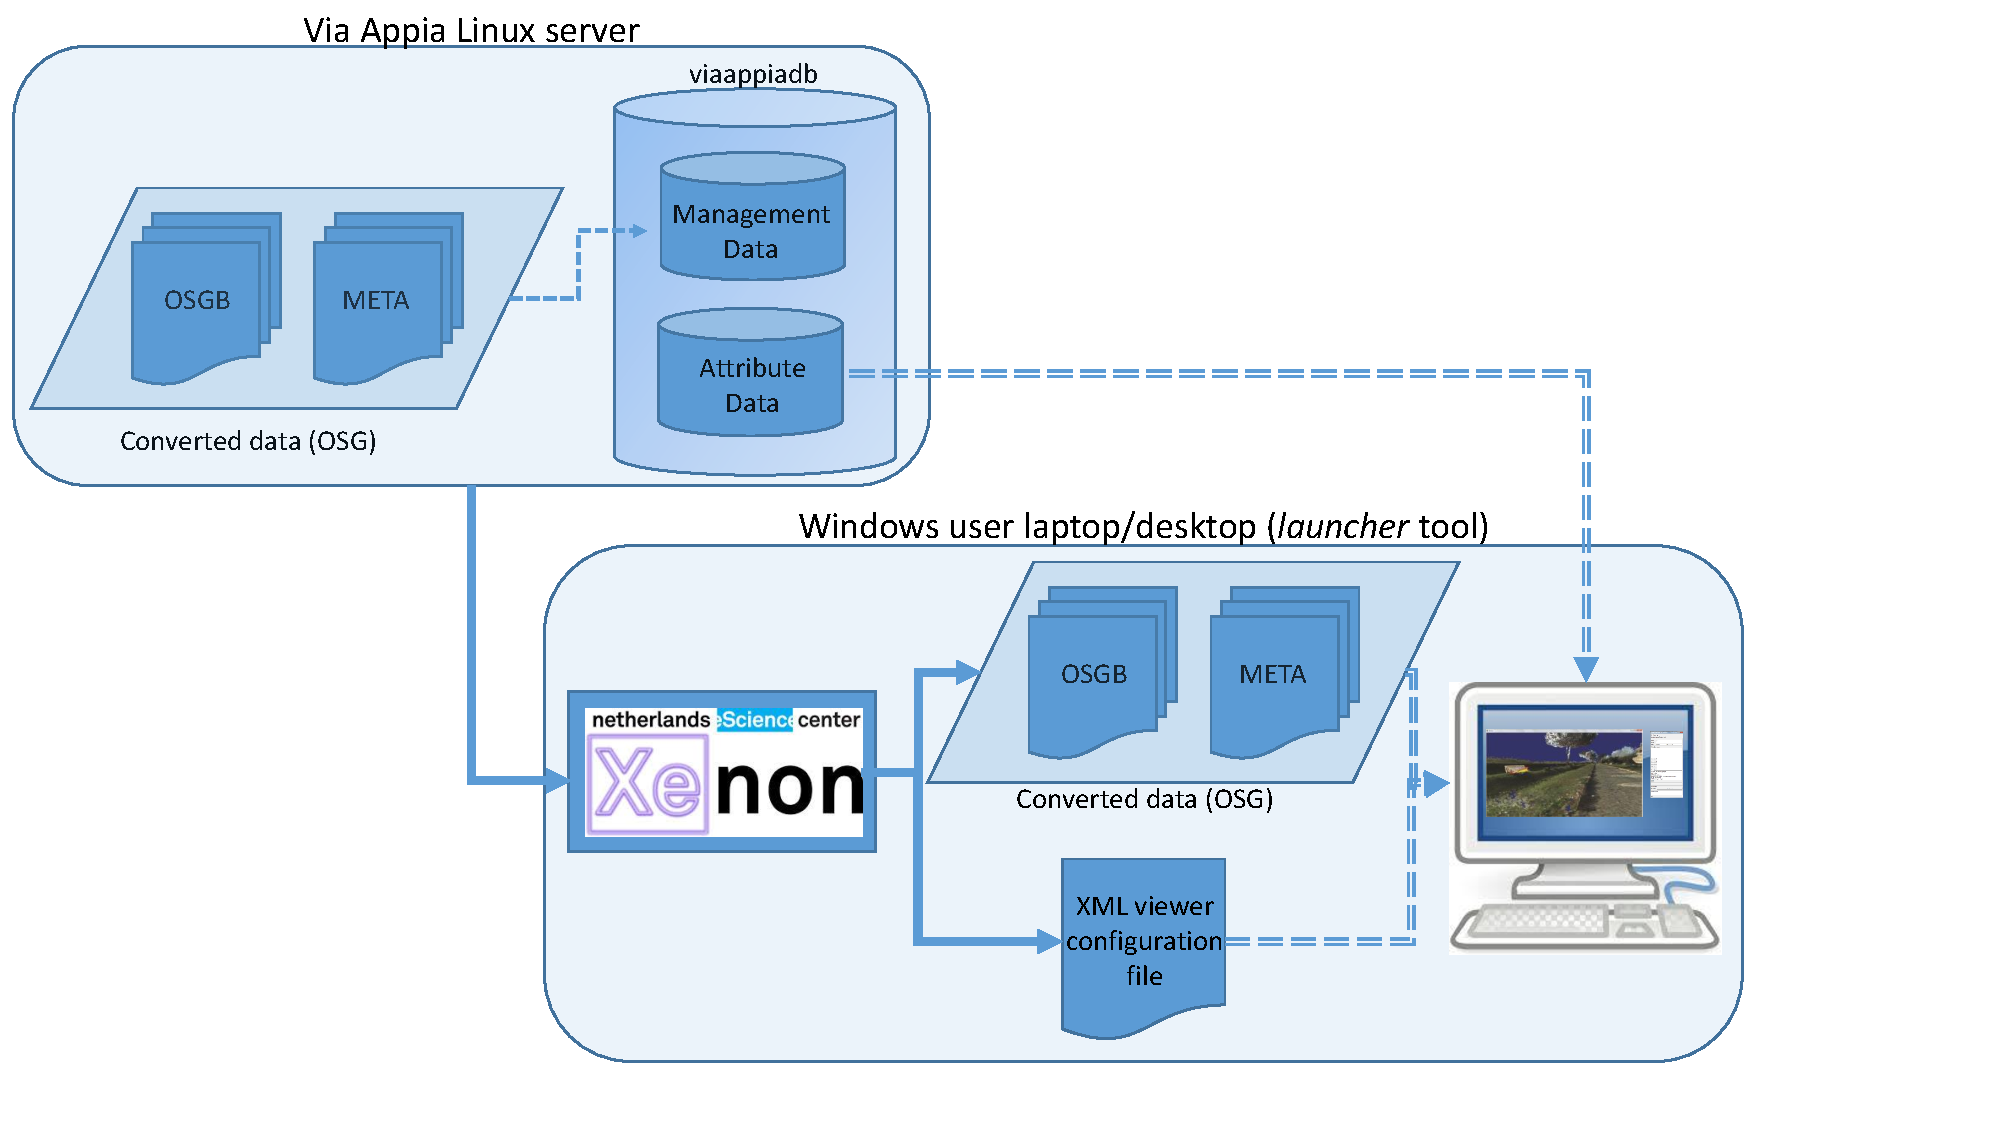
\includegraphics[scale=0.5]{fig/communication.pdf}
\caption{Two-tier architecture of the Via Appia 4D GIS and the steps executed in the clients (launcher tool).}
\label{fig-communication}
\end{figure}

Both the execution of the data preparation framework in the server and the data synchronization steps in the client (\textit{launcher} tool) have been automated. In order to use the new 4D GIS system the end-user only needs to do:
\begin{itemize}
\item (a.) Obtain an account in the Via Appia Linux server and in the \textit{viaappiadb} database and generate a SSH key pair (see Subsections \ref{sec:accounts} and \ref{sec:sshkeys}).
\item (b.) Download, install and configure the \textit{launcher} tool in his Windows laptop or desktop (see Subsection \ref{sec:install}).  The \textit{launcher} tool also contains the 4D viewer. It is also recommend to install two tools for the communication between the Linux server and the Windows computers: PuTTY and WinSCP (see Subsubsections \ref{sec:putty} and \ref{sec:winscp}).
\end{itemize}

\section{Via Appia Linux server}
\label{sec:server}

The Via Appia Linux server contains the master copy of the data and the \textit{viaappiadb} database. Any user attempting to use the Via Appia 4D GIS system must have access to the server and to the database.

\subsection{Specifications}

The Via Appia server is rented from Hetzner (http://www.hetzner.de). The specifications of the server are:

\begin{itemize}
\item OS: CentOS 6.5 64 bit
\item 1 x CPU: Intel 8 Cores i7-4770 CPU @ 3.40GHz
\item Memory: 32 GB
\item Storage:
\begin{itemize}
\item Western Digital RE WD2000FYYZ 2TB 64MB Cache SATA 6.0Gb/s (mounted in /home)
\item 2 x Intel SSDSC2BW240A4 530 Series 240GB in RAID 1 (mounted in /, /boot and SWAP)
\end{itemize}
\item Network: 
\begin{itemize}
\item RealTek RTL-8169 Gigabit Ethernet driver
\item IP: 148.251.106.132
\end{itemize}
\end{itemize}

\subsection{Linux - Windows communication}
\label{sec:com}
The server is a Linux system while the clients use Windows computers. There are many options in the market for the communication between Linux and Windows systems but for the Via Appia 4D GIS system we use the tools described in the following Subsubsections.

\subsubsection{Windows SSH client}
\label{sec:putty}

In order to have a command-line environment we connect to the server through ssh. From another Linux system the server can be reached with:

\begin{Verbatim}[fontfamily=courier,commandchars=\\\{\},fontsize=\footnotesize]
ssh \textit{userName}@148.251.106.132
\end{Verbatim}

For Windows systems it is advisable to download and install PuTTY (http://www.putty.org) in order to get a terminal-like environment. The IP of the Linux server (148.251.106.132) and your user name in the server are required.

\subsubsection{Windows SCP client}
\label{sec:winscp}

For simple data transfers between Windows systems and Linux systems and vice versa we recommend to download and install WinSCP (http://winscp.net). The IP of the Linux server (148.251.106.132) and your user name in the server are required.

\subsubsection{Xenon}

When executing the 4D viewer in the Windows computer the required data is automatically downloaded from the Linux server. The \textit{launcher} tool is in charge of this task and it is based on the NLeSC Xenon library (http://estep.esciencecenter.nl/index.php/component/k2/item/1-xenon).

\subsection{Accounts}
\label{sec:accounts}

In order to obtain an account in the server the system administrator must be contacted (o.rubi@esciencecenter.nl). In addition, an account specific for the \textit{viaappiadb} database should also be created. Usually both accounts have the same name.

After your account in the server has been created you can already connect to the server with ssh, through PuTTY in Windows systems. 

Once the database account has been created and you are connected to the server you can access the DB locally using the \textit{psql} client. You need to set your PostgreSQL password (which can be different to your operative system password). You can set your PostgreSQL password with (replacing \textit{username} with your PostgreSQL user name and \textit{password} with a password of your choice):

\begin{Verbatim}[fontfamily=courier,commandchars=\\\{\},fontsize=\footnotesize]
psql -c "alter user \textit{username} WITH PASSWORD '\textit{password}'";
\end{Verbatim}

The \textit{viaappiadb} database can also be accessed using \textit{phpPgAdmin}. With an internet browser connect to \textit{http://148.251.106.132/phpPgAdmin}. The generic user is \textit{viaappia} and the generic password is \textit{peileed0woh7AhY3}. Next you also need to specify your PostgreSQL user and password.

\subsection{SSH keys}
\label{sec:sshkeys}

For the proper working of the 4D GIS system a SSK key pair has to be created in the Via Appia Linux Server. The steps are:

\begin{itemize}
\item Connect to the Via Appia Linux server. Use PuTTY in Windows systems.
\item Create a key pair:
\begin{Verbatim}[fontfamily=courier,commandchars=\\\{\},fontsize=\footnotesize]
ssh-keygen -t rsa
\end{Verbatim}
 Press \textit{Enter} three times to use the default configuration (Important: Do not provide a passphrase).
\item Add the public key to the authorized keys:
\begin{Verbatim}[fontfamily=courier,commandchars=\\\{\},fontsize=\footnotesize]
cat ~/.ssh/id_dsa.pub >> ~/.ssh/authorized_keys
\end{Verbatim}
\item Change permissions to the \textit{.ssh} directory and its contents:
\begin{Verbatim}[fontfamily=courier,commandchars=\\\{\},fontsize=\footnotesize]
chmod 600 ~/.ssh/
chmod 600 ~/.ssh/*
\end{Verbatim}
\end{itemize}

After the key pair has been generated in the Via Appia Linux server you need to download a copy of the private key to your Windows computer. You need this key when configuring \textit{launcher} tool.  We recommend to use the clipboard together with PuTTY:
\begin{itemize}
\item Connect to the Via Appia Linux server from your Windows computer with PuTTY.
\item Once your are connected open the private key file:
\begin{Verbatim}[fontfamily=courier,commandchars=\\\{\},fontsize=\footnotesize]
less ~/.ssh/id_rsa
\end{Verbatim}
\item Select all the text of the key and ``copy'' it (right button of the mouse and click on \textit{Copy}). Be sure that you have selected all the key, we recommend to maximize the window.
\item Create an empty text file in your Windows machine (for example in \textit{Documents}) and ``paste'' the private key.
\item Save the file and name it \textit{id\_rsa}.
\end{itemize}

\section{Data}
\label{sec:data}

The types of data that the Via Appia 4D GIS system deal with are:

\begin{itemize}
\item A low resolution point cloud of the research area that has been generated making use of Fugro’s DRIVE-MAP services. 
\item High resolution point clouds and meshes of the different objects of interest (sites) generated using photogrammetric technologies. 
\item Sites reconstructions (meshes) for different epochs. 
\item Historical pictures or paintings. 
\item Attributes information for the sites and their parts, which are gathered by field observations, such as composition, condition, interpretation, description of the different elements, etc. 
\end{itemize}

However, the data needs to be converted to the OpenSceneGraph binary format which is used by the 4D viewer. Hence, we do a distinction between raw data and OSG (converted) data. The master copy of the data is in the Via Appia Linux server where also the database required by the system is running. When new raw data is available, for example a new point cloud for a certain site or a new reconstruction of a site, it is required to add it to the raw data locations in the Via Appia Linux server. After adding the new data in the server location for the raw data we need to run the part of the data preparation framework that converts the data into the OSGB format and updates the \textit{viaappiadb} database with the latest changes. For this purpose we use the Python script called \textit{createosgdata.py}.

There are certain rules regarding the data that need to be followed for the correct functioning of the system. They are described in the following sections. Please, read them carefully.

All the data is stored in the directory \textbf{\textit{/home/vadata/DATA}}. Only the user \textbf{\textit{vadata}} has permission to modify the content of the data directory. Therefore, before adding new raw data we have to change from our user to the \textit{vadata} user. Once connected in the Via Appia Linux server we can become the \textit{vadata} user with:

\begin{Verbatim}[fontfamily=courier,commandchars=\\\{\},fontsize=\footnotesize]
ssh vadata@localhost
\end{Verbatim}

Only certain users can currently use the \textit{vadata} user: Oscar Martinez Rubi, Stefan Verhoeven, Maurice de Kleijn and Rens de Hond.

One usual use case is when we have new data in our Windows machine. In such case use WinSCP to transfer the data from your Windows systems to your home directory in the Via Appia Linux server. Then, close WinSCP and use PuTTY to connect to the server in a terminal-like environment. The first thing you need to do is become the \textit{vadata} user. Next you have to copy the added data to the proper location in the directory \textit{/home/vadata/DATA/RAW}.

\subsection{Raw data}

The raw data is \textbf{only} stored in the Via Appia Linux server and there is Python script that needs to be used to generate the converted OSG data, the \textit{createosgdata.py}. The raw data directory is \textit{/home/vadata/DATA/RAW}. In the next Subsubsections we give more information about the different types of raw data. All the data locations are relative to the directory \textbf{\textit{/home/vadata/DATA/RAW}}.

\subsubsection{Background point cloud}

Using the DRIVE-MAP service of Fugro the fifth and sixth miles of the Via Appia were scanned and a point cloud was produced. The spatial reference system of this data is EPSG:32633. The resolution of this point cloud is not enough to see detailed features and the sites were only scanned from the main road. Thus, the back of the sites is missing.

The background LAS files are stored in \textit{PC/BACKGROUND/DRIVE\_1\_V3}. In the folder \textit{PC/BACKGROUND} there must be only one sub-folder (currently DRIVE\_1\_V3). If a new version of the DRIVE-MAP is used you must delete the previous one (or moved it out of this directory).

About the names of the background sub-folders, they can not contain dots, so valid names are for example DRIVE\_1\_V3.

\subsubsection{Sites}
\label{sec:sites}

For the different sites (objects of interest in the area) several type of data are also used.

\paragraph{Point clouds}

Higher resolution point clouds must be stored in the directory \textit{PC/SITES}. This directory contains different folders for each site. For example the folder  \textit{PC/SITES/162} contains LAS files of different point clouds of site 162. 

The LAS files contained in each site subfolder may have been pre-aligned (using CloudCompare for example). In that case the LAS file name must be \textbf{*\_aligned\_\textit{BGNAME}*} where \textit{BGNAME} must be the background name (as contained in the folder \textit{PC/BACKGROUND/}).
Some point clouds generation tools store the color information in 8 bits instead of the usual 16 bits. In that case the file name must be \textbf{*\_8bitcolor*}. The effect of having an undeclared LAS file with 8 bit color is that the converted data will be black and white. Note that these properties are cumulative, for example \textit{162\_aligned\_DRIVE\_1\_V3\_8bitcolor.las} is a valid name for a LAS file with 8 bit color information and aligned points.

\paragraph{Meshes}

The meshes are stored in the directory \textit{MESHES}. There are two types of meshes: (a.) current  mesh representations of the sites, and (b.) archeological reconstructions. They must be stored respectively in \textit{MESHES/CURR} and \textit{MESHES/ARCH\_RECONS}. Each of these directories contains different folders for each site. For example the folder \textit{MESHES/CURR/162} contains mesh representations of the current state of the site 162. 

For each site there must be different folders for the several meshes. Inside these folders the files for the meshes are stored (OBJ, MTL, JPEG). For example \textit{MESHES/CURR/162} could contain two folders called \textit{162\_curr\_1} and \textit{162\_curr\_2} and each of them contain a OBJ, a MTL and several JPEG files. 

Similarly to the LAS files the meshes can also be aligned. In this case the folder name for a certain mesh must be \textbf{*\_aligned\_\textit{BGNAME}*}. 

\paragraph{Pictures}

The pictures are stored in the directory \textit{PICTURES}. There are two types of pictures: (a.) pictures of the current state of the sites, and (b.) historical pictures or even paintings. They must be stored respectively in \textit{PICTURES/CURR} and \textit{PICTURES/HIST}. Each of these directories contains different folders for each site. For example the folder \textit{PICTURES/CURR/162} contains pictures of the current state of the site 162. Note that in this case these folders directly contain the images similarly to the point clouds but contrary to the meshes where the folder for each site contains subfolders.

\paragraph{Attributes data (Microsoft Access file)}

The attribute information gathered in the field is stored in a Microsoft Access file. The content of this file has to be imported into the \textit{viaappiadb} database. In order to do this conversion we recommend to use the tool \textit{Bullzip Access to PostgreSQL} which is available for Windows machines. The steps for the conversion are:

\begin{itemize}
\item Install in a Windows system:
\begin{itemize}
\item Microsoft Access.
\item Bullzip Access to PostgreSQL (http://www.bullzip.com/products/a2p/info.php).
\end{itemize}
\item If the format of the file is not \textit{.mdb} we recommend to reformat the file. If this is required follow these steps (example for Microsoft Access 2010):
\begin{itemize}
\item Open the Access file.
\item Click Save and Publish.
\item Click on save database as Access 2002-2003 database.
\end{itemize}
\item Execute the converter:
\begin{itemize}
\item Select the Access file.
\item If there is an error message about a missing driver, just follow the recommended instructions.
\item Select create dump file.
\item Leave all the default values except creating indexes. Disable it because otherwise it would create indexes with erroneous names.
\item Run the converter.
\end{itemize}
\item We still need to do some modifications to the generated SQL dump file:
\begin{itemize}
\item Remove the \textit{CREATE DATABASE} statement in the beginning of the file.
\item Remove any default values in all columns with type TIMESTAMP.
\item Remove all the double quotes (").
\item Be careful with possible table names with blank spaces (which should be removed).
\item Remove all index creations (if you did not de-select the index creation). 
\end{itemize}

\item Once the PostgreSQL dump file is generated, use WinSCP to transfer the file to the Via Appia Linux server.
\item Use PuTTY to log in into the server and become the \textit{vadata} user.
\item Move the SQL dump file to the \textit{ACCESS} folder.
\item Still with the \textit{vadata} user execute the Python script \textit{mergeaccess.py} to update the Attribute information in the \textit{vadata} database. Note that the attribute tables of the \textit{viaappiadb} database will be overwritten.
\end{itemize}

\paragraph{Footprints}

The footprints SQL dump file has to be put in the directory \textit{FOOTPRINTS}. The table in this file has to be called \textit{sites\_geoms\_temp} and contain (at least) the columns \textit{site\_id} and \textit{geom}. To import a new footprints file use the Python script \textit{mergefootprints.py}

\subsection{OSG}

The raw data needs to be converted to the OSGB format. For that purpose we have created the Python script \textit{createosgdata.py}. This script should be run with the \textit{vadata} user and should be run when some data has changed in the raw data directory.

In order to view the data in your Windows machine you need to download a version of the converted OSG data in your local machine. We use a NLeSC tool called Xenon.

\subsection{Data structure overview}
\label{sec:structoverview}

The data stored in the Via Appia Linux server follows a certain data structure which has been introduced in the previous Subsubsections. In Figure \ref{fig:dataover} we show the data structure overview, the folders and files in \textbf{bold} are within the defined structure while the ones in \textit{italic} are examples. Only the \textit{RAW} folder is analysed because it is in the raw locations where the users can make modifications, the \textit{OSG} folder is automatically handled by the system.

\begin{figure}
\begin{Verbatim}[fontfamily=courier,commandchars=\\\{\},fontsize=\footnotesize, frame=lines]
\textbf{DATA}
  |- \textbf{RAW}                  
  |   |- \textbf{PC}
  |   |   |- \textbf{BACKGROUND}
  |   |   |     |- \textit{DRIVE_1_V3}
  |   |   |          |- \textit{1.las}
  |   |   |- \textbf{SITES}
  |   |   |     |- \textit{162}
  |   |   |         |- \textit{162_aligned_DRIVE_1_V3_8bitcolor.las}
  |   |- \textbf{MESHES}
  |   |   |- \textbf{CURR}
  |   |   |     |- \textit{162}
  |   |   |         |- \textit{162_aligned_DRIVE_1_V3}
  |   |   |             |- \textit{162_aligned_DRIVE_1_V3.obj}
  |   |   |- \textbf{ARCH_RECONS}
  |   |- \textbf{PICTURES}
  |   |   |- \textbf{CURR}
  |   |   |     |- \textit{162}
  |   |   |         |- \textit{162_current.png}
  |   |   |- \textbf{HIST}
  |   |- \textbf{ACCESS}
  |   |   |- \textbf{attributes.sql}
  |   |- \textbf{FOOTPRINTS}
  |   |   |- \textbf{footprints.sql}
  |- \textbf{OSG}                  
      |- \textbf{PC}
      |   |- \textbf{BACKGROUND}
      |   |- \textbf{SITES}
      |- \textbf{MESHES}
      |   |- \textbf{CURR}
      |   |- \textbf{ARCH_RECONS}
      |- \textbf{PICTURES}
      |   |- \textbf{CURR}
      |   |- \textbf{HIST}
      |- \textbf{DOMES}
      |- \textbf{BOUNDINGS}
\end{Verbatim}
\caption{Data structure overview}
\label{fig:dataover}
\end{figure}

\newpage

\section{Database}
\label{sec:db}

The \textit{viaappiadb} database is running in the Via Appia Linux server. See Subsection \ref{sec:accounts} on how to get an account in the database. The database is a PostgreSQL 9.2.8 instance running with PostGIS 2.1.2.

This database has two categories: (a.) data management information and (b.) the attribute data. In next Subsections we describe each category. In Figure
\ref{fig:erviaappiadb} we show the Entity-Relationship diagram of the \textit{viaappiadb}.

\begin{figure}[!ht]
\centering
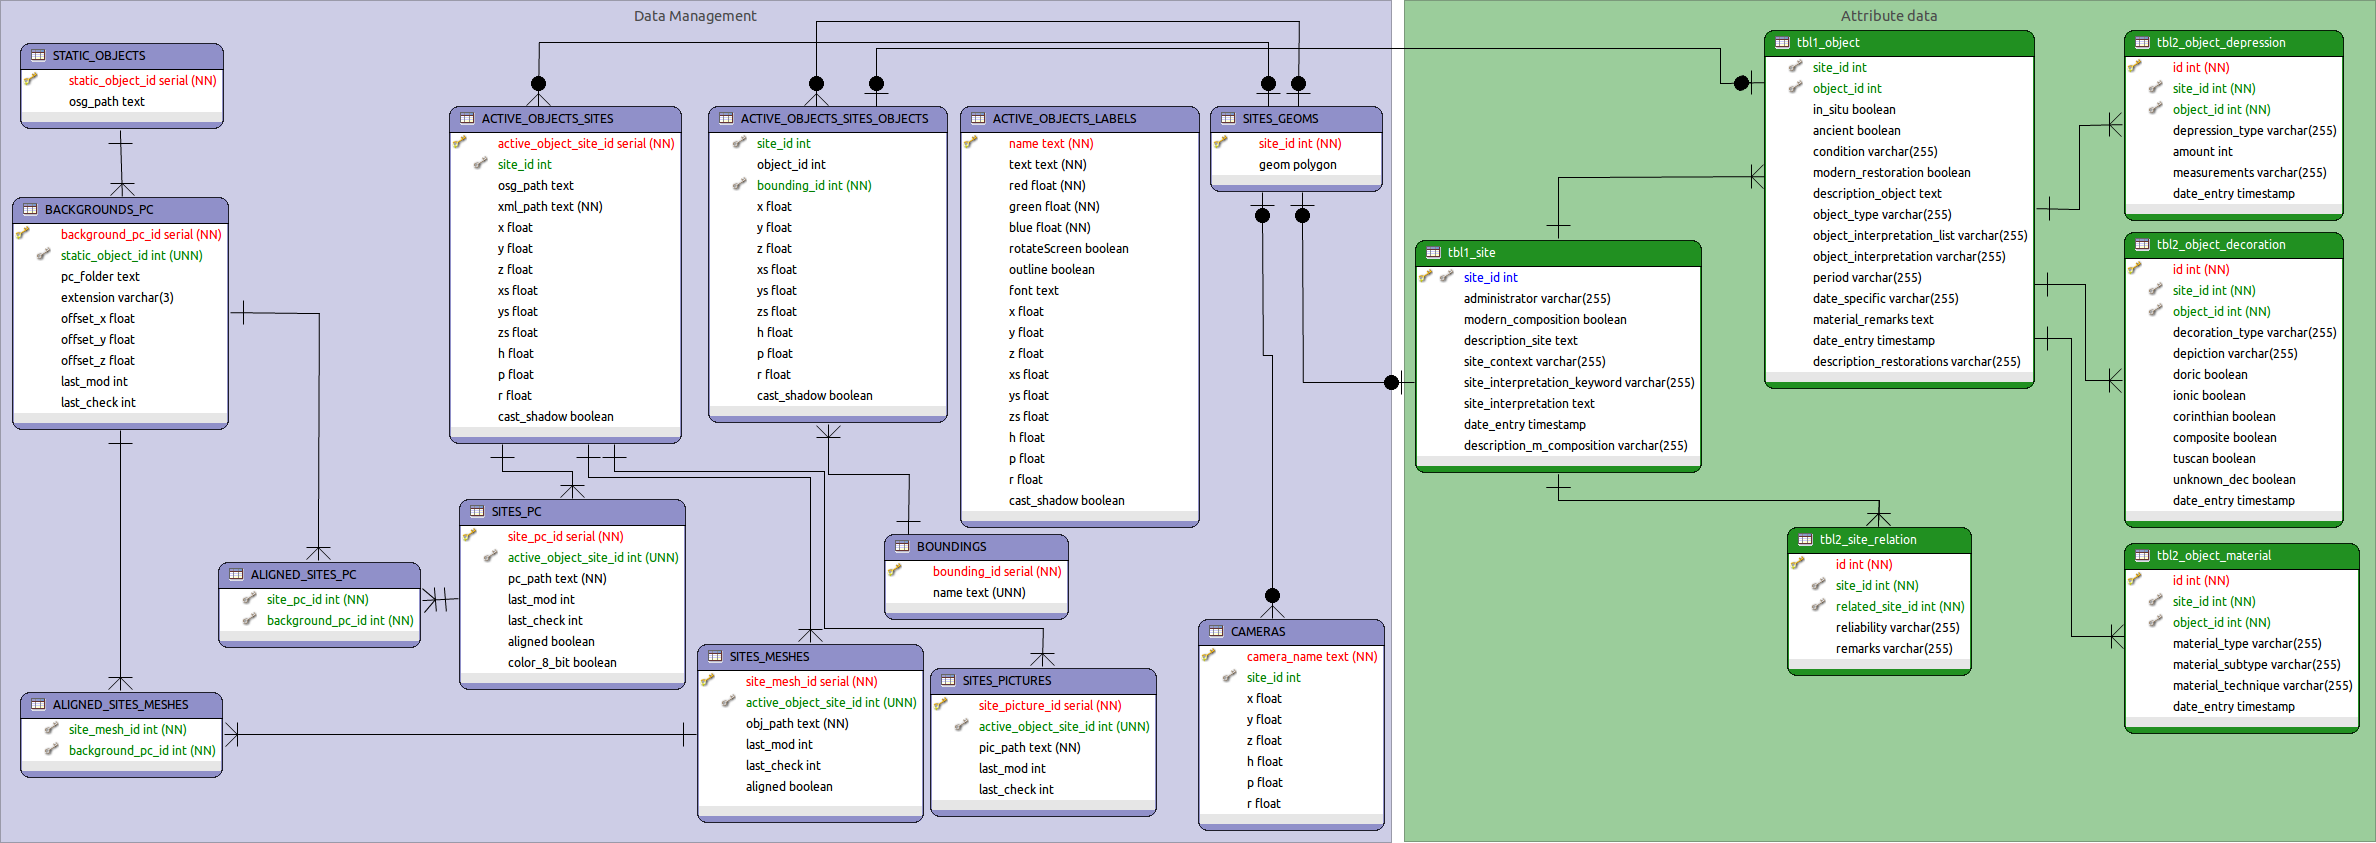
\includegraphics[width=\textwidth]{fig/ERDB}
\caption{Entity-Relationship diagram of the \textit{viaappiadb} with its two categories}
\label{fig:erviaappiadb}
\end{figure}

Note that some of the nodes of the relationships are \textit{0..n} or \textit{0..1} (with black points) instead of the usual \textit{1..n} or \textit{1..1}. This is to illustrate that some sites and objects may have entries in some tables but not in others. For example it is possible to have a site in the attributes table (tbl1\_site) that does not have any entry in the footprints table (sites\_geoms).

\subsection{Data management}

This category contains tables with the locations of the raw and converted data, visualization-related data and the footprints of the sites.

\begin{itemize}
\item Raw data: BACKGROUNDS\_PC, SITES\_PC, SITES\_MESHES and SITES\_PICTURES contain the locations of the different types of raw data, concretely the low resolution point cloud of the background and the per-site high resolution point clouds, meshes and pictures. They also contain information about aligned point clouds and meshes (ALIGNED\_SITES\_PC and ALIGNED\_SITES\_MESHES) and 8-bit-colors in point clouds.

\item Converted data: STATIC\_OBJECTS and ACTIVE\_OBJECTS\_SITES contain the locations of the converted background point cloud and the converted per-site data, i.e. high resolution point clouds, meshes and pictures. The data of these tables is used in visualization.

\item Visualization-related data: ACTIVE\_OBJECTS\_SITES\_OBJECTS contains the different positions of the bounding boxes around the objects of the sites. Note that we consider the site itself to be an object as well, in this case it is the object with \textit{object\_id -1}. There are different types of bounding boxes listed in table BOUNDINGS. ACTIVE\_OBJECTS\_LABELS and CAMERAS have information about labels added into the 4D scene and camera positions respectively.

\item Footprints: The table SITES\_GEOMS contains footprints of different sites.
\end{itemize}

The raw data is maintained and modified with the user \textit{vadata} (see Section \ref{sec:data}) while the converted data is generated with the \textit{createosgdata.py} script. This tool also generates some visualization-related data which can be modified and extended through the 4D viewer. The footprints can be updated with the \textit{mergefootprints.py} Python script.

\subsection{Attribute data}

The attribute data is a direct import from the Microsoft Access file that contains the attribute information for the sites. See the paragraph regarding the Attribute data in Subsection \ref{sec:sites} to see how to import the Microsoft Access file into the \textit{viaappiadb}. Note that every time that a new Attribute file is imported the tables are overwritten.

\section{Via Appia Windows launcher and 4D viewer}
\label{sec:viewer}

Before being able to run the viewer, we need to download the data from the Via Appia Linux server to the user Windows computer. Not all the data is required, only the converted data is actually used for the visualization. The \textit{launcher} tool takes care of (a.) synchronizing the data between the two systems, (b.) starting the 4D viewer, and (c.) updating the \textit{viaappiadb} with possible changes done with the viewer (for example a repositioning of a mesh).

\subsection{Installation}
\label{sec:install}

The GitHub repository in https://github.com/NLeSC/Via-Appia contains all the available software. Download the code either by cloning the repository with Git software or by downloading a ZIP (in the repository URL clink on ``Download ZIP''. If you do not have access to the repository contact Oscar Martinez Rubi, Stefan Verhoeven, Maurice de Kleijn or Rens de Hond.

Once you have acquired the ViaAppia software you can find the \textit{launcher} tool in the directory launcher/binary/ViaAppia.bat. 

\subsection{Requirements}

The launcher requires the JAVA SE development kit:
\begin{itemize}
\item Browse to http://www.oracle.com/technetwork/java/javase/downloads/index.html
\item Download the Java SDK.
\item Install it (follow the instructions).
\end{itemize} 

The 4D viewer requires the 2012 and 2013 Microsoft Visual Studio C++ Redistributable. You can either download them or use the installers which are already provided in the ViaAppia software in the directory viewer/EXT\_LIB. In addition you should download the latest drivers for your graphics card.

\subsection{Configuration}

After solving the requirements both the \textit{launcher} and the 4D viewer are ready to work. However, the \textit{launcher} needs to be configured.

In launcher/binary directory you need to create a file called config.properties (Important: be careful with hidden extensions). You can use as template the provided config\_template.properties. We recommend to ``Copy-Paste'' the file and rename the new file to config.properties. Open the file and fill in your details:

\begin{itemize}
\item Replace the tag \textless{}UserRemote\textgreater{} with your user name in the Via Appia Linux server.
\item Replace the tag \textless{}UserLocal\textgreater{} with your user name in your Windows computer.
\item Replace the tag \textless{}localPrivateKey\textgreater{} with the file name of the private key that you copied from the Linux server. If you have not done this yet see Subsection \ref{sec:sshkeys}.
\item In the template file we assume that you are storing all the Via Appia in:
\begin{verbatim}
C:\\Users\\<UserLocal>\\ViaAppia
\end{verbatim}
If that is not the case you may need to explicitly change some other properties.
\item In the template file we also assume that the root directory of the Via Appia software is in:
\begin{verbatim}
C:\\Users\\<UserLocal>\\ViaAppia\\Via-Appia-master
\end{verbatim}
If that is not the case you need to change the \textit{viewer} property.
\item Note that in some properties the separation between folders is done with / and in others is done with \textbackslash{}\textbackslash{}. For each property use the same format as in the template file.
\end{itemize}

\subsection{Execution}

Once the configuration is properly filled in you can execute the \textit{launcher} tool with the script in launcher/binary/ViaAppia.bat. 

The execution of this tool will synchronize the data from the Via Appia server into your Windows computer and will download the latest configuration file required by the viewer.
% (see Appendix \ref{sec:xmlconfig} for more information regarding the viewer configuration file). 
When the synchronization is done, the viewer is automatically started. 

Once you are done with the viewer be sure to save the progress. After closing the several windows in the screen the \textit{launcher} tool will ask you if you want to commit your changes to the \textit{viaappiadb}.

\subsection{4D Viewer API}

The \textit{launcher} tool starts the 4D viewer after the synchronization of the data is finished. Two windows are visible: one with the 4D scene and the other one with the GUI which contains four tabs. In the next Subsubsections we describe each of these tabs. By clicking on the Help button in the GUI main menu bar a more detailed help text can be displayed (only in Dutch). 

In order to load the data into the scene we need to open the XML configuration file. Click on File and Open, navigate to the folder where the data has been downloaded and select the ViaAppia.conf.xml file (the default is /Users/\textless{}UserLocal\textgreater{}/ViaAppia/DATA/OSG/ViaAppia.conf.xml).

This will load the 4D scene and some data will already be visible in the visualization window. By default only the low resolution background point cloud is visible. This data is static and can not be moved, resized or rescaled. For each site there can be different pictures, meshes and point clouds. These are active objects which are not visible by default but when they become visible they can be moved, resized and rescaled.

A very important characteristic of this GIS system is that each site is identified by its bounding cube. Within each site we can also identify objects or parts of the sites which are also defined by their bounding cubes. The bounding cubes (for a site or for the parts of a site) are also active objects, i.e. they can be moved, resized and rescaled. As the other types of active objects, they are not visible by default.

\subsubsection{Main tab}

After loading the configuration file the the main tab of the GUI looks like Figure \ref{fig-guimain}. 

\begin{figure}[!ht]
\centering
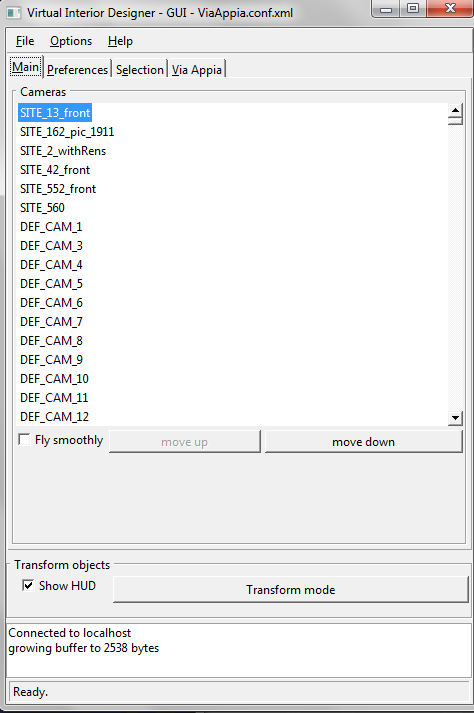
\includegraphics[scale=0.5]{fig/main}
\caption{Via Appia 4D viewer GUI: main tab}
\label{fig-guimain}
\end{figure}

This tab lists all the camera positions. The user can add new camera positions. Click on the mouse right-button on top of the cameras list and select ``Create new''. The cameras can be related to a certain site. If that is the case the camera name must start with \textit{SITE\_XXX} where \textit{XXX} is the site identifier. For the sites without user-defined camera positions a default camera position is generated based on the sites footprints.

\subsubsection{Preferences tab}

The preferences tab looks like Figure \ref{fig-guipref} and it has some visualization options that can be modified. The most important one is the Level of detail. Computers with low visualization resources (without powerful GPU cards) should run with lower Level of detail. Hence, if you experience a non smooth visualization try to decrease the Level of detail.

\begin{figure}[!ht]
\centering
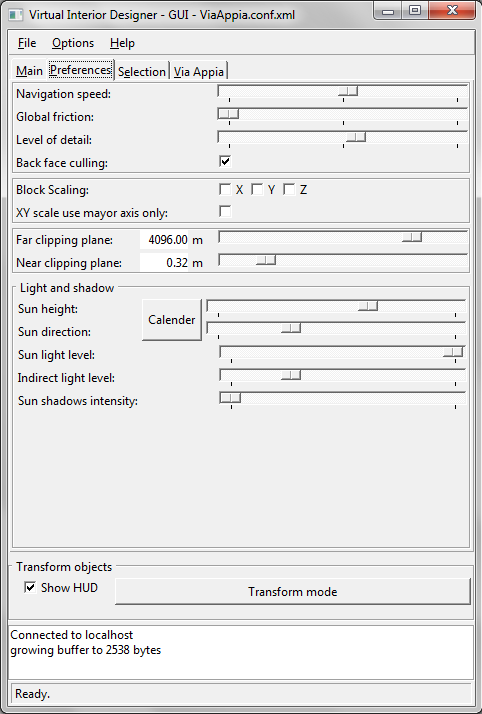
\includegraphics[scale=0.5]{fig/preferences}
\caption{Via Appia 4D viewer GUI: preferences tab}
\label{fig-guipref}
\end{figure}

The speed of the navigation is also configurable.

\subsubsection{Selection tab}

Clicking the ``t'' key activates the Transform mode. In this mode we can modify the position, size and rotation of active objects, i.e. points clouds, meshes and pictures related to the sites, and also their bounding cubes and bounding cubes of their parts / objects. In addition we can use the \textit{ruler} tool. Moreover we can add labels into the 4D scene and define new bounding cubes for new parts or objects within sites. See section \ref{sec:guiname} for more information about adding new labels and bounding cubes.

When you select an active object in the 4D scene, its details appear in the Selection tab as for example shown in Figure \ref{fig-guisel}. The active object can be moved, resized and rotated directly in the visualization of by specifying the values in the Selection tab (very useful when doing large changes).

\begin{figure}[!ht]
\centering
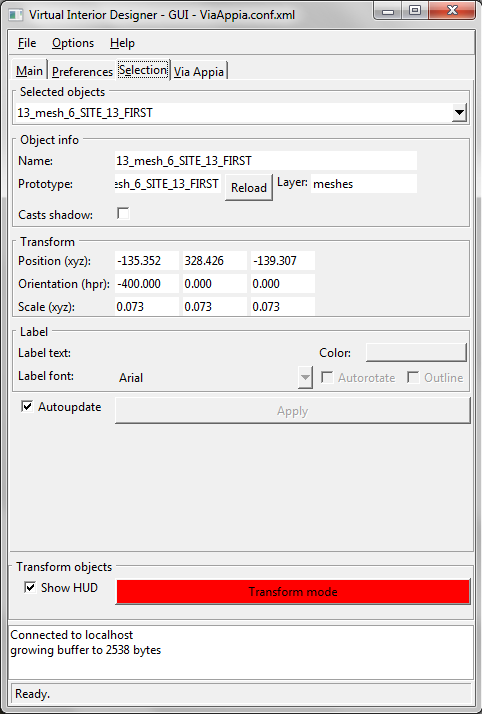
\includegraphics[scale=0.5]{fig/selection}
\caption{Via Appia 4D viewer GUI: selection tab}
\label{fig-guisel}
\end{figure}

\subsubsection{Via Appia tab}

\begin{figure}[!ht]
\centering
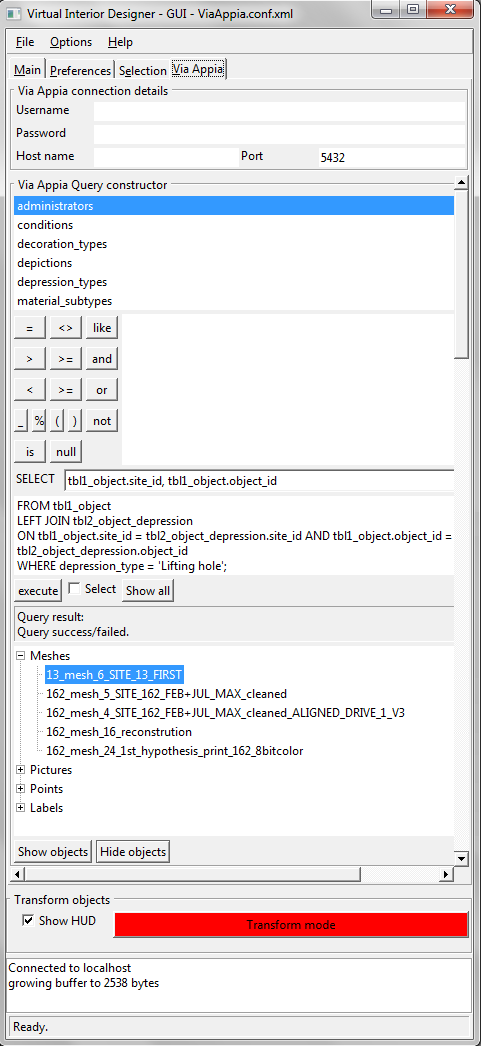
\includegraphics[scale=0.5]{fig/viaappia}
\caption{Via Appia 4D viewer GUI: Via Appia tab}
\label{fig-guiva}
\end{figure}

The last tab is called Via Appia. It is used to toggle the visibility of the different active objects. It contains two parts: 
\begin{itemize}
	\item The \textit{viaappiadb} connector. SQL statements can be constructed to access the Attributes data of the \textit{viaappiadb}. The selected columns of the SQL statement must be \textit{site\_id} or \textit{site\_id,object\_id}. After a SQL statement has been constructed and the connection details have been properly filled up it is executed in the remote DB. The bounding cubes related to the selected sites and objects (parts) will become visible in the 4D scene. If there is only one site or part selected in the DB and the \textit{select} check-box is checked in the GUI, the bounding box is selected in the 4D scene and it can be modified (see Selection tab).
	\item The active objects tree. The rest of active objects (point clouds, meshes, pictures and labels) are listed and can be showed or hidden in the 4D scene.
\end{itemize}

Note that even if different active objects become visible the user will only see them if the camera position is pointing at them. To change the camera position use the main tab.

\subsubsection{Naming rules}
\label{sec:guiname}

For the proper functioning of the system there are some rules that must be followed when adding new cameras, labels or bounding boxes:

\paragraph{Cameras}

By default one camera is created per site and it is located in the center of the footprint of the site. The users can create new cameras but their names must start with \textit{SITE\_XXX} if they are related to a certain site.

\paragraph{Labels}
 
When adding a new label the \textit{Name} (in the Object info box) must contain be \textit{*label*}. When a label is related to a site we suggest to use a name like \textit{SITE\_XXX\_label}. The \textit{Label text} (in the Label box) can contain any text.

\paragraph{Boundings}

The different objects or parts of a site are identified by an \textit{objectId}. We consider that the site itself is a object or part of the site, in this case it is the \textit{objectId} -1. 
When adding a bounding for a new site use the ``t'' key to enable the Transform mode. Use the last option to add a bounding box and move it and rescale it to contain the site you want. The \textit{Name} (in Object info in Selection tab) must be \textit{[siteId]\_obj\_-1}.

When adding a new bounding box for a object or part of a site the \textit{Name} must be \textit{[siteId]\_obj\_[objectId]}. For example 162\_obj\_10. Please be sure that the \textit{objectId} that you choose is not being already used. To see if it is used you can use the \textit{viaappiadb} connector. For example by executing the SQL query \textit{SELECT 162,10;} (and checking the Select check-box) you can see if there is already a object defined with id 10 for the site 162. 

\subsubsection{Unsynchronized 4D viewer}

If you wish to start the viewer without data synchronization you can do it directly with the script in viewer/viewer/startViewer.bat. However, note that since the synchronization is deactivated this will start the viewer with probably older data and a older configuration file. In addition, in this mode the changes done in the scene are not automatically committed to the \textit{viaappiadb}. Therefore, we discourage using the viewer/viewer/startViewer.bat.

%\appendix

%\section{4D viewer XML configuration file}
%\label{sec:xmlconfig}

%\subsection{Creating a XML configuration file}

%\subsection{Updating the database with a XML configuration file}

%\section{Python scripts}
%\label{sec:python}

\end{document}

